\chapter{Reliability and Quality }
\section{Reliability Physics}
\subsection{Introduction and General Thermodynamics}
Quality refers to the property of the CMOS to work as intended without failing. Reliability is quality measured over time. Thus, reliability is a measure of the fabricated CMOS to function properly during its life. 

\noindent Our fabricated devices are prone to several failure mechanisms, for example, capacitor leakage in an IC leads to its failure. Reliability physics studies the kinetics of failure mechanisms whereas reliability engineering refers to the practices to reduce failure probability such as: proper design rules, material selection, manufacturing guidelines etc.

\begin{figure}[htb]
\centering
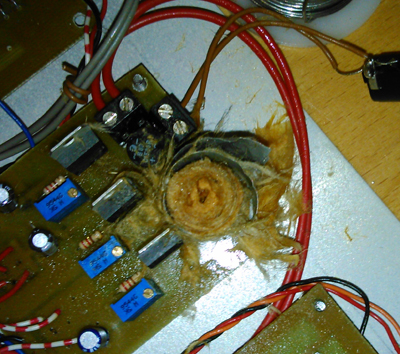
\includegraphics[scale=0.6]{./fig26} % e.g. insert ./image for image.png in the working directory, adjust scale as necessary
\caption{A capacitor that has broken down due to dielectric leakage}
\label{3.26} % insert suitable label, this is used to refer to a fig from within the text as shown above
\end{figure}

As a consequence of Moore’s law, there is a steady decrease in device size with every technology node which implies a higher current density and electric field. Thus, even during normal use a device is close to its breakdown state as the operating voltage isn’t scaled linearly with the size. Reliability studies of a device are therefore of great importance.
One might wonder, why does a device fail? In fact, most of the devices that we use are metastable i.e they are stable now but are prone to fail in the future. Devices fail because according to thermodynamics, all systems tend to assume the most stable state (possessing zero potential energy) however input energy is required to bring about this change. The Gibb’s potential is a good measure of a device’s internal energy. Let us consider a capacitor, electric field does work against conservative forces to polarize the dielectric. This increases the Gibb’s energy of the dielectric and it therefore wishes to assume a state of lower Gibb’s energy which it achieves via dielectric breakdown that lowers its internal energy to zero thus allowing it to assume a stable state.
\subsection{Hazard function}
Hazard function, h(t) is the instantaneous failure rate of a device. It tells us the number of devices that will fail, mean time-to-failure and expected number of failures in an interval. There are different types of hazard functions: constant, linearly increasing, decreasing etc, representing differing failure rates. 

For a given data, we have f(t) which is our p.d.f for failure that tells us number of failures between t and t+dt, F(t) as cumulative fraction that tells us total number of failures until t. R(t) is a measure of devices that work till time t. It is a measure of reliability. R(t)+H(t)=1 always. Hazard function is ratio of failure pdf to R(t).

\section{Reliability Statistics}
In order to determine the reliability of devices, statistics plays a crucial role as it allows us to determine a device’s lifetime, plot and visualize device data and study about their reliability, failure etc. There are three curves of importance to us; Gaussian and Lognormal distribution: used for fitting reliability data for failure due to processes like corrosion, and Weibull distribution for fitting data for weakest link failure modes.


\pagebreak
\subsection{Gaussian, Lognormal and Weibull Distribution}
Gaussian distribution is widely used for time-to-failure modelling of devices that fail due to failure modes such as corrosion. We determine the cum-fraction for each data point after arranging them in ascending order and plot Z (standard deviation) as a function of time. We get a straight-line graph with Z=0 corresponding to median (time at which 50% of the devices fail) and Z=-1 as the time at which 16% devices fail. The difference between median and the latter gives us the standard deviation. Now that we know the mean and the standard-deviation we can plot the p.d.f as a function of time to get a gaussian distribution.

\begin{figure}[htb]
\centering
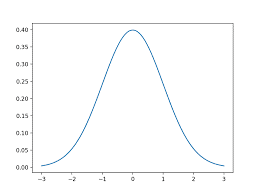
\includegraphics[scale=0.6]{./fig27} % e.g. insert ./image for image.png in the working directory, adjust scale as necessary
\caption{A gaussian distribution}
\label{3.27} % insert suitable label, this is used to refer to a fig from within the text as shown above
\end{figure}

\noindent Using the data, we can calculate instantaneous survival failure rate and average failure rate. Lognormal distribution is plotted similarly but by using a different plotting function.

\begin{figure}[htb]
\centering
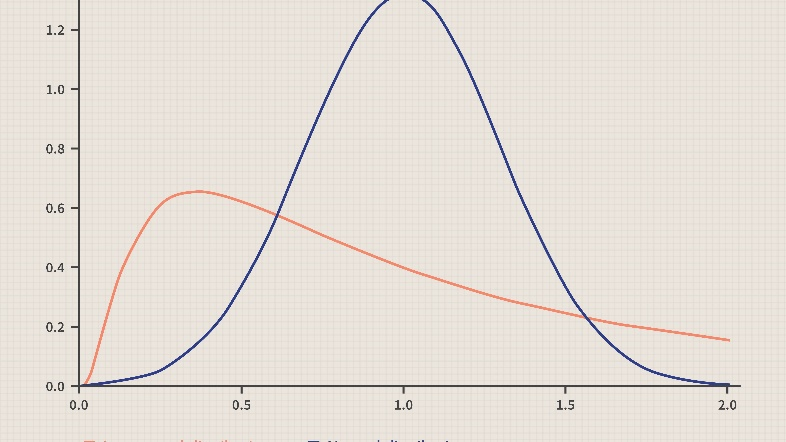
\includegraphics[scale=0.6]{./fig28} % e.g. insert ./image for image.png in the working directory, adjust scale as necessary
\caption{A lognormal distribution}
\label{3.28} % insert suitable label, this is used to refer to a fig from within the text as shown above
\end{figure}

\noindent Weibull function is used for weakest link modelling and is characterized by two parameters: time-to-failure and shape parameter. Differing values for shape parameter give us different curves allowing us to determine device stability.

\begin{figure}[H]
\centering
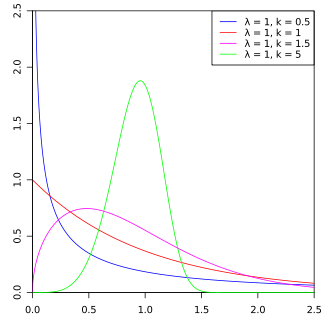
\includegraphics[scale=0.6]{./fig29} % e.g. insert ./image for image.png in the working directory, adjust scale as necessary
\caption{Weibull distribution. Differing values of shape parameter give us different graphs gaussian, exponential etc}
\label{3.28} % insert suitable label, this is used to refer to a fig from within the text as shown above
\end{figure}




\section{Bathtub Curve for Reliability }

\begin{figure}[htb]
\centering
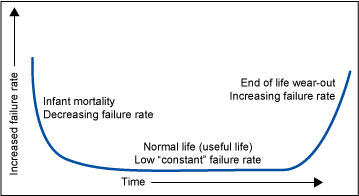
\includegraphics[scale=0.6]{./fig30} % e.g. insert ./image for image.png in the working directory, adjust scale as necessary
\caption{The bathtub curve}
\label{3.30} % insert suitable label, this is used to refer to a fig from within the text as shown above
\end{figure}


\noindent Bathtub curve is a curve that fits hazard function or failure rate as a function of time. It has three regions: EFR (Early-Failure Rate), IFR (Intrinsic-Failure Rate) and the Wear-out region. 
EFR: this region corresponds to an exponentially decreasing hazard function. This region symbolizes a very high-failure rate reducing drastically with time. In electronics, this may be due to manufacturing defects resulting in low-breakdown strength etc. 
A device can last for a year in the EFR under operating conditions. In order to remove the device from EFR region, we put it under increased stress to accelerate the time-to-failure process and this period is known as burn-in. The burn-in period is used to push the device through a year of its lifetime, if it is defective it fails during the burn-in period. The burn-in allows to remove devices from EFR and enter IFR.


\noindent IFR: this region corresponds to a low and constant hazard function. The failure rate is low and constant for a long period of time. Failure can occur in this region due to small defects.
Wear-out region: In this region, the failure rate increases monotonically with time. Failure occurs due to wear-out mechanisms resulting from long-term usage, for example, dielectric failure.
To understand the bathtub curve, we can take the example of human life. When we are born, the first year as an infant is very important and utmost care is taken. This is because infants have a very high mortality rate. Infant Mortality Rate is a concern for all societies. We take utmost care of the infant when it is born to ensure that the baby is healthy as any form of disease can be fatal. Once the baby grows up, the mortality rate is relatively very low and we don’t have to worry about our health as we did for the baby. There are few chances of us being struck by a fatal disease, we live for a long time working healthily. But as we get older, our body becomes weaker and once again we become susceptible to ailments of the old age that keep getting worse with time.
We were in the EFR as a baby, in the IFR as a boy and a man and in the Wear-out region as an old man.



